\documentclass[aps,prd,10pt,onecolumn,nofootinbib,superscriptaddress,floatfix]{revtex4-2}

\usepackage[T1]{fontenc}
\usepackage{lmodern}
\usepackage[utf8]{inputenc}
\input{glyphtounicode}
\pdfgentounicode=1
\usepackage{amsmath,amssymb,mathtools}
\usepackage{bm}
\usepackage{graphicx}
\usepackage{placeins}
\usepackage{hyperref}

\hypersetup{
  colorlinks=true,
  linkcolor=blue,
  citecolor=blue,
  urlcolor=blue
}

\begin{document}
\raggedbottom

\title{Can a Wormhole Induce a Monopole?}

\author{Sergei Slobodov}
\email{sergei@slobodov.com}
\noaffiliation

\date{\today}

\begin{abstract}
Could a body orbiting near one mouth of a traversable wormhole make the mass
seen near the other mouth rise and fall?  We show that to first order in the
source mass, the vacuum Einstein equations on a Schwarzschild background hold
the mass monopole around the far mouth fixed for any motion of the source, while the higher multipoles do
respond.  The periodic monopole signal proposed for searches around Sgr~A*
is therefore absent.  Beyond first order, the Bondi mass of an isolated far mouth can
decrease through radiation but cannot increase, even with an evolving throat;
for two mouths in one universe, the same conclusion follows in the limit of
large separation, assuming the geometry has a regular limit.  The
electromagnetic counterpart is exact: the charge seen through a closed surface
changes only if current crosses it.  The local results require neither a
compact interior nor an asymptotic end.
\end{abstract}

\maketitle

\section{Introduction}
\label{sec:introduction}

Seen from far away, the mouth of a traversable wormhole looks like any other
compact mass.  One way to tell it apart would be to detect influence from the
other side: fields reach through the throat, so matter moving near the far
mouth should leave some imprint on orbits near ours.  Dai and Stojkovic (DS)
proposed a concrete version of this idea
\cite{DaiStojkovic2019Observing}.  In their model, two Schwarzschild exteriors
are joined at a throat of radius $R$, and a mass $\mu$ is placed at radius $A$ in
one of them.  Solving the static problem gives a mass shift $b=\mu R/A$ seen
from the other exterior.  Letting $A$ follow an eccentric orbit then makes
this mass rise and fall, producing a periodic $1/r^2$ acceleration of nearby
stars.  Simonetti et al.\ \cite{SimonettiEtAl2021SensitiveSearches} and
Moiseev and Sazhina \cite{MoiseevSazhina2025ObservationalSearch} have used
this signal to design searches around Sgr~A*.

The monopole is special, however.  In electrostatics, the charge seen through
a closed surface can change only if charge crosses that surface, whether or
not the surface encloses a compact region.  Fields of higher multipoles pass
through a wormhole throat freely, but the monopole flux through each mouth is
fixed.  The DS calculation solves a static problem at each source position and
then lets the position vary, so the question is whether this sequence of
static solutions is an allowed evolution.  In this note we show that, for the
monopole, it is not.

We make only a few assumptions:
\begin{itemize}
\item The measuring surface around the observer's mouth lies in vacuum, so
  no matter crosses it.  This is the situation DS consider: the source stays
  on the other side.
\item For the first-order result, the background near the observer is
  Schwarzschild, as in the DS model, and the source mass is small,
  $\mu/M\ll1$.
\item For the result beyond first order, the observer's end is
  asymptotically flat and vacuum near future null infinity, so that its Bondi
  mass is defined.  When both mouths open into one universe, we assume in
  addition that the geometry has a regular limit as their separation grows.
\end{itemize}

Sections~\ref{sec:maxwell}--\ref{sec:nonlinear} treat the charge, the
first-order mass and the Bondi mass in turn, and the Appendix estimates the
quadrupolar field that does reach the observer.

\subsubsection*{Relation to earlier work}

For a spherically symmetric configuration, Krasnikov pointed out that
Birkhoff's theorem already excludes the DS signal
\cite{Krasnikov2020CommentObserving}.  Our first-order result extends this to
nonspherical source motion, and the Bondi argument extends it beyond first
order.  The choice of monopole sector behind the DS signal also appears in
Copson's potential for a charge near a black hole, which Linet corrected in
the same way (Sec.~\ref{sec:maxwell}).

We use $G=c=1$ and $r_g=2M$, where $M$ is the background Schwarzschild mass.

\section{Conservation of electric monopole charge}
\label{sec:maxwell}

In the DS electrostatic model, two flat exteriors are joined at $r=R$,
with charge $q$ at $r_1=A$ in one exterior.  Let $c_1,c_2$ be the
asymptotic potentials.  Matching the potential and its normal derivative
gives the field in the other exterior,
\begin{equation}
 V_2=c_2+\sum_{\ell\ge0}\frac{B_\ell}{r_2^{\ell+1}}
 P_\ell(\cos\theta_2),\qquad
 B_{\ell\ge1}=q\,\frac{2\ell+1}{2(\ell+1)}
 \frac{R^{2\ell+1}}{A^{\ell+1}},\qquad
 B_0=\frac{qR}{2A}+\frac{R}{2}(c_1-c_2).
 \label{eq:ds-multipoles}
\end{equation}
Here $P_\ell$ is a Legendre polynomial and the observer-side charge is
$Q_2=B_0$.  The source position fixes the higher multipoles but not the
monopole, since $c_1-c_2$ is independent boundary data.
DS set $c_1=c_2$, obtaining $Q_2=qR/(2A)$
\cite{DaiStojkovic2019Observing}.

Let $F$ be the electromagnetic field strength, $j$ the electric current
one-form, and $\star$ the Hodge dual.  On a closed measuring surface $S$,
define
\begin{equation}
 Q[S]=\frac{1}{4\pi}\int_S\star F.
 \label{eq:maxwell-charge}
\end{equation}
A family of such surfaces sweeps out a timelike worldtube $\mathcal T$
with boundary $S_{t_2}-S_{t_1}$.  Integrating $d\star F=4\pi\star j$
and applying Stokes' theorem gives
\begin{equation}
 Q[S_{t_2}]-Q[S_{t_1}]=\int_{\mathcal T}\star j.
 \label{eq:maxwell-balance}
\end{equation}
Without current across $\mathcal T$, the charge is constant.
This is exact even on an evolving metric and requires neither a compact
interior nor an asymptotic end.  Electromagnetic radiation carries
energy, not charge.  Frolov and Novikov established this flux balance
for wormholes, and Krasnikov solved the fixed-flux problem for a point charge
\cite{FrolovNovikov1990PhysicalEffects,Krasnikov2008ElectrostaticInteraction}.
The same local balance applies to a one-ended handle, where the counterpart
of $c_1=c_2$ is a single-valued potential.  Conserving the flux instead
gives the static field a circulation around a loop through the throat and
back through the exterior, about $q/A$ when the mouths' separation $D$
through the exterior is much larger than $A$
(Fig.~\ref{fig:fixed-sector-field}) \cite{FrolovNovikov1990PhysicalEffects}.

\begin{figure}[!htbp]
  \centering
  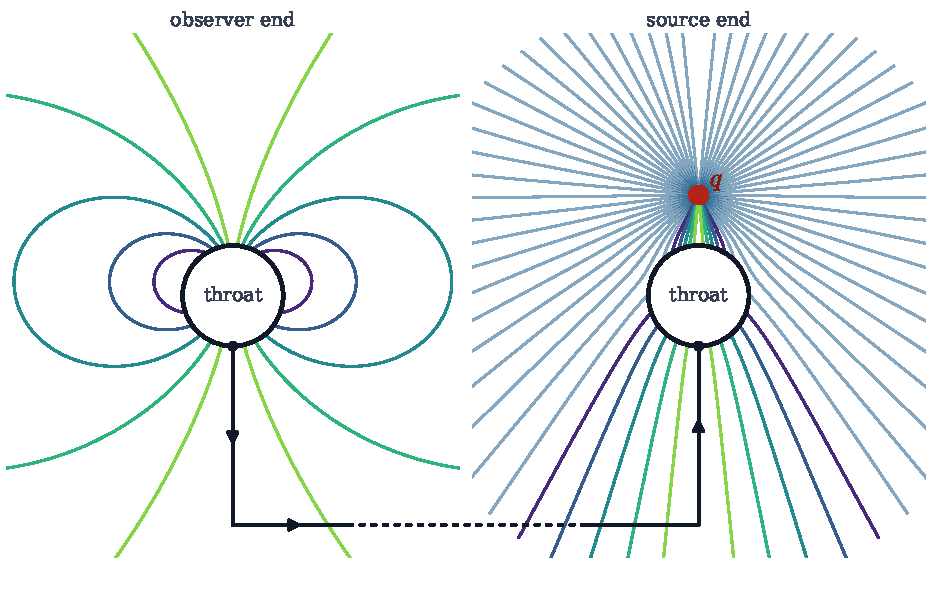
\includegraphics[width=0.82\textwidth]{figures/fig_thinshell_fixed_monopole_flux_v12.pdf}
  \caption{The zero-flux member of Eq.~\eqref{eq:ds-multipoles}: $B_0=0$,
  requiring $c_2-c_1=q/A$.  The black circles represent the same throat sphere
  in the two exterior charts.  Field lines cross the throat but return through
  another angular band, giving zero net flux.  The
  observer-side field is nonzero and contains only $\ell\ge1$ terms.
  For a one-ended handle with widely separated mouths, the panels show the
  neighborhoods of the two mouths.  The directed loop enters the throat in
  the source chart, leaves at the same point in the observer chart, and
  returns through the shared exterior (dotted); the field has circulation
  $q/A$ around it.}
  \label{fig:fixed-sector-field}
\end{figure}

Imposing $c_1=c_2$ anew as $A$ changes selects different charges, not
successive states of a no-current evolution.  The DS relation $Q_1+Q_2=q$, with $Q_1$ the
source-side flux, conserves only the sum, whereas
Eq.~\eqref{eq:maxwell-balance} conserves each charge separately when
neither measuring worldtube is crossed.

The monopole sector is fixed by the history of the system, not by
conditions imposed at infinity; the black hole is the classic example.
Copson's potential for a static point charge $q$ at radius $A$ outside a
Schwarzschild black hole \cite{Copson1928} leaves the hole with the charge
$-qM/A$.  Linet removed it with the source-free monopole that keeps the hole
neutral \cite{Linet1976}, and Smith and Will computed the self-force in this
sector \cite{SmithWill1980}.  With two ends the same problem takes the form
$c_1=c_2$: requiring $V=0$ at both ends fixes the voltage between them, and
with it a far-end charge that follows the source.
In Eq.~\eqref{eq:ds-multipoles}, the source-free term
$\tfrac{R}{2}(c_1-c_2)$ plays the role of Linet's monopole:
Eq.~\eqref{eq:maxwell-balance} holds $Q_2$ fixed, and $c_1-c_2$ adjusts as
the source moves.  A self-force calculation for a spherical thin-shell
wormhole makes this choice, so its wormhole charge changes with the source
position, which no evolution without current allows \cite{RubinDeCelis2013}; with
Linet's correction, its far-field force becomes the Smith--Will value for a
black hole of the same mass at leading order.  Boisseau and Linet noticed the
free monopole coefficient but left it undetermined
\cite{BoisseauLinet2013Electrostatics}.  In the cylindrical model the far-end
flux does not depend on the source position, so the static family can
describe an evolution \cite{RubinDeCelisSimeone2020}.

Fixed monopole flux does not eliminate the transmitted field:
Fig.~\ref{fig:fixed-sector-field} shows a nonzero observer-side field
with $B_0=0$.

\section{Constancy of the first-order mass monopole}
\label{sec:gravity}

In the DS construction the Schwarzschild exteriors have
$d\bar s^2=-f\,dt^2+f^{-1}dr^2+r^2d\Omega^2$, with
$f=1-r_g/r$, and are joined at $R>r_g$.
In their revised preprint, the observer-side static perturbation is
\cite{DaiStojkovic2019ObservingV3}
\begin{equation}
 h^{\mathrm{obs}}_{tt}=\frac{2b}{r_2},\qquad
 h^{\mathrm{obs}}_{rr}=\frac{2br_2}{(r_2-r_g)^2},\qquad
 b=\frac{\mu R}{A}.
 \label{eq:ds-observer-mode}
\end{equation}
Both components give
$h^{\mathrm{obs}}_{\alpha\beta}=b\,\partial_M\bar g_{\alpha\beta}$:
$b$ is a mass shift, with far-field acceleration $-b/r_2^2$.
At first order about Schwarzschild the harmonic sectors decouple, and every
vacuum $\ell=0$ perturbation is a constant mass shift plus a coordinate
change \cite{MartelPoisson2005SchwarzschildPerturbations}, whatever the
source's motion.

\begin{samepage}
Promoting $A$ to $A(t)$ makes this perturbation the linearization of
the metric above with $f$ replaced by
$F(t,r_2)=1-2[M+b(t)]/r_2$.  The linearized mixed Einstein component is
\begin{equation}
 \delta G^r{}_t=\frac{2\dot b}{r_2^2}
 =-\frac{2\mu R\dot A}{A^2r_2^2}.
 \label{eq:momentum-constraint}
\end{equation}
Vacuum therefore requires $\dot b=0$: the proposed monopole modulation
vanishes.  The constant mass shift is fixed by the initial data, not by
the instantaneous orbital radius.
In spherical symmetry, Krasnikov identified this obstruction using
Birkhoff's theorem \cite{Krasnikov2020CommentObserving}.
\end{samepage}

A time-dependent gauge term cannot supply an observable mass change.
The argument is local to the observer's vacuum region; it assumes
neither vacuum at the throat nor any asymptotic structure.
Higher multipoles remain possible.  Using Sgr~A*/S2 length scales, the
static stiff-shell calculation in Appendix~\ref{app:quadrupole} gives a
quadrupolar acceleration scale of order
$10^{-8}$ times the proposed monopole scale.  Repeated passages could
exceed this estimate if they resonantly excite a weakly damped quadrupolar
mode \cite{CardosoFranzinPani2016Ringdown}.

\section{Nonincrease of the observer-end mass}
\label{sec:nonlinear}

For a two-ended asymptotically flat wormhole, let $E_B(u)$ be the observer
end's Bondi energy: the asymptotic mass monopole in a fixed Bondi frame.
With regular Bondi asymptotics and vacuum near that end's future null
infinity, the standard exact balance law is
\cite{BondiVanderBurgMetzner1962Gravitational,Sachs1962Asymptotic,
WaldZoupas2000Conserved}
\begin{equation}
 E_B(u_2)-E_B(u_1)
 =-\frac{1}{32\pi}\int_{u_1}^{u_2}du
    \int_{S^2}N_{AB}N^{AB}\,d\Omega\le0,
 \qquad u_2>u_1.
 \label{eq:bondi-integrated}
\end{equation}
Here $N_{AB}=\partial_u C_{AB}$ is the Bondi news, with
$g_{AB}=r^2q_{AB}+rC_{AB}+O(1)$, $q^{AB}C_{AB}=0$, and angular indices
raised with the inverse $q^{AB}$ of the unit-sphere metric $q_{AB}$.
Thus $E_B$ cannot rise even if
the source and throat evolve nonlinearly; no energy condition on the
supporting matter is needed.  The DS mass $E_B=M+\mu R/A(u)$ rises as the
source approaches the throat and fails this test.  Source motion may still
modulate the rate of radiative loss.

When both mouths share one asymptotic region, its Bondi energy belongs
to the whole system, not to either mouth.  Increasing the exterior
separation suppresses the influence between the mouths through ordinary
space while retaining their connection through the throat.

Suppose a family with exterior
mouth separation $D$ and a fixed source--throat experiment converges
smoothly on every compact spacetime region containing the source, throat,
and corresponding fixed-radius observer-side cuts to a two-ended
spacetime with the above asymptotics.  Let $E_H^{(D)}(u,r)$ be the quasilocal
Hawking energy of such a cut.  Smooth convergence at fixed $r$, followed by
$r\to\infty$ along asymptotically round outgoing cuts, gives the Bondi
energy of the limiting observer end \cite{MarsSoria2015HawkingEnergy}:
\begin{equation}
 \lim_{r\to\infty}\lim_{D\to\infty}E_H^{(D)}(u,r)
 =E_B^{\mathrm{lim}}(u).
 \label{eq:one-ended-limit}
\end{equation}
The limiting observer-end mass is therefore nonincreasing; the argument
gives no finite-separation or finite-radius bound.

\section{Conclusion}
\label{sec:conclusion}

The charge seen through a closed surface around a mouth changes only when
current crosses it.  On a Schwarzschild background, the first-order mass
monopole is constant in the vacuum region around the observer's mouth,
whatever the motion of the source.  Beyond first order, the Bondi mass of an
observer end that is vacuum near future null infinity can decrease through
radiation but cannot increase; for mouths sharing one exterior, the same
holds in a regular limit of large separation.

The DS signal arises from reading a family of static solutions, each in its
own monopole sector, as an evolution.  As in Linet's correction of Copson's
potential, the homogeneous monopole places the solution in the sector fixed
by the charge actually present.  For a thin-shell wormhole this sector
changes the far-field self-force to the black-hole value at leading order.

Higher multipoles do reach the observer through the throat.  For Sgr~A*, the
static stiff-shell estimate of the quadrupole is of order $10^{-8}$ of the
proposed signal.  Repeated passages could exceed this estimate if they
resonantly excite a weakly damped quadrupolar mode, and source motion may
modulate radiative mass loss.  A bound at finite mouth separation remains
open.

\begin{acknowledgments}
The author thanks Ilia Slobodov for helpful discussions.
\end{acknowledgments}

\section*{Artificial Intelligence Use Statement}

The author used OpenAI ChatGPT/Codex and Anthropic Claude as interactive
assistants for brainstorming, mathematical and editorial critique, prose
revision, consistency checks, reference searches, and figure preparation.  All
arguments, calculations, citations, figures, and conclusions were reviewed and
revised by the author, who is solely responsible for the manuscript.

\appendix
\section{A quasistatic quadrupole benchmark}
\label{app:quadrupole}

We estimate the quasistatic tidal response as the source moves.  At first
order about Schwarzschild, the even-parity $\ell=1$ vacuum mode is a
locally pure-gauge displacement; the odd-parity mode is a constant
angular-momentum shift \cite{MartelPoisson2005SchwarzschildPerturbations}.
The first local, gauge-invariant time-dependent vacuum field is therefore
quadrupolar \cite{Thorne1980Multipole}, unlike the Maxwell dipole in
Fig.~\ref{fig:fixed-sector-field}.

We compare its quasistatic acceleration with the proposed monopole scale
$a_{\mathrm{DS}}\sim\mu R/(Ar_2^2)$.
In the tidal approximation, the quadrupolar part of the source potential
at the throat scales as $\mu R^2/A^3$, and the transmitted potential
decays as $(R/r_2)^3$.
Radial differentiation therefore gives
\begin{equation}
 \frac{a_2}{a_{\mathrm{DS}}}
 \sim C_2\left(\frac{R}{A}\right)^2
          \left(\frac{R}{r_2}\right)^2.
 \label{eq:quadrupole-benchmark}
\end{equation}
To calculate $C_2$, use the static stiff-shell construction of
Ref.~\cite[Appendix~D.1]{CardosoEtAl2017LoveNumbers}.  Its polar metric
amplitudes on the source and observer sides are
$H_0^{(s)}=\alpha P_2^2(x)+\beta Q_2^2(x)$ and
$H_0^{(o)}=\gamma Q_2^2(x)$, where $x=r/M-1$; no applied tide is present
on the observer side.  With the surface-density perturbation set to zero,
the angular metric amplitude $K$ and its derivative along the continuous
tortoise coordinate are continuous at the throat.  Equivalently,
\begin{equation}
 \frac{\gamma}{\alpha}
 =\frac12\left(\frac{K_P}{K_Q}-\frac{K_P'}{K_Q'}\right)_{r=R},
 \qquad
 C_2=\frac85\left(\frac{M}{R}\right)^5\frac{\gamma}{\alpha}.
 \label{eq:quadrupole-transfer}
\end{equation}
Here $K_P,K_Q$ follow from the cited relation between $K$ and $H_0$ by
inserting $P_2^2,Q_2^2$, respectively; primes denote outward $r$ derivatives.
The normalization follows from $P_2^2(x)\sim3x^2$,
$Q_2^2(x)\sim8/(5x^3)$ and the factor three from radial differentiation.
This gives $0<C_2<5/2$ for $R>2M$, approaching $5/2$ in the weak-field
limit and zero as $R\to2M$.

For favorable Sgr~A*/S2 parameters $A\sim R\sim r_g$,
$r_g\simeq0.084\,\mathrm{AU}$ and $r_2\simeq1000\,\mathrm{AU}$,
the geometric factor in Eq.~\eqref{eq:quadrupole-benchmark} is
$7\times10^{-9}$.  With $C_2<5/2$, the quasistatic stiff-shell model
gives $a_2/a_{\mathrm{DS}}\lesssim2\times10^{-8}$.
The near-mouth substitution is an order-of-magnitude extrapolation of
the tidal scaling, not an exact orbital calculation.
We retain $R-r_g\gg\mu$ for perturbative consistency.

\bibliographystyle{apsrev4-2}
\bibliography{references,references_v11_additions,references_v12_preview}

\end{document}
